\chapter{Design}
This section will cover the details of the methods and algoithms that were used in the implementation of the project. The previous section covered the history of some of these techniques which were imperative for building the foundation of the methods described in this chapter.

Deep Q-Networks and its enhancements have the majority of focus, as it is the basis of the project. Below is a table of the different experiments and the methods that were used in order to produce the best solution for each tested environment.

\begin{table}[h!]
	\begin{center}
		\begin{tabular}{|c|c|c|}
			\hline
			Network   & Algorithm                  & Environment    \\
			\hline
			CNN + MLP & Q-Learning                 & Pong           \\
			CNN + MLP & Q-Learning                 & Breakout       \\
			CNN + MLP & Duelling Double Q-Learning & Space Invaders \\
			\hline
		\end{tabular}
		\caption{Best performing method in given environment}\label{table:design:algo-experiment}
	\end{center}
\end{table}

\section{Markov decision process}
\label{dsgn:sec:mdp}
This section will describe some of the basics of Markov decision processes (MDP), they are the foundation of the reinforcement learning methods that will be described later in this chapter. First, we need some mathematical definitions of MDPs, these are from David Silver's excellent lecture series on Reinforcement Learning.

Markov decision processes are just markov reward processes with decisions, i.e. At each state $S_t$, we have a finite set of actions to choose from in order to get to a new state $S_{t+1}$.

\begin{defn}
	A Markov decision process is a tuple $\langle \mathcal{S}, \mathcal{A}, \mathcal{P}, \mathcal{R}, \gamma \rangle$.
	\begin{itemize}
		\item $\mathcal{S}$, finite set of states
		\item $\mathcal{A}$, finite set of actions
		\item $\mathcal{P}$, state transition probability matrix,~\\$\mathcal{P}_{ss'}^a = \mathbb{P}[S_{t+1}=s'|S_t=s, A_t=a]$
		\item $\mathcal{R}$, reward function, $\mathcal{R}_s^a = \mathbb{E}[R_{t+1}|S_t=s,A_t=a]$
		\item $\gamma$ discount factor, $\gamma\in[0,1]$
	\end{itemize}
\end{defn}

The definition above defines a Markov decision process, which we use as a basis for describing the methods in reinforcement learning. In order to illustrate the idea, let us consider the game of Pong. For simplicity, assume we can encode each frame of the game into the set of states $\mathcal{S}$. In order to play the game, we need to know what the best action to take would be at each frame of the game to move the paddle under the ball, hitting the ball back and (hopefully) scoring a point.

Given a frame of the game $S_t$ and the set of actions we can choose from $A_t$, we are going to try and maximise our future (expected) reward using the reward function $\mathcal{R}_{S_t}^{A_t}$. We want to choose the best action $a$, that will result in the maximum future reward. It is important that we don't look at immediate rewards only, since, in Pong we don't get the point until we have hit the ball back to the other side.

In order to look at future rewards, we use the discount factor $\gamma$. When $\gamma$ is close to zero, we are ``\textit{myopic}'' in our evaluation (we only look for short-term rewards). However, as $\gamma$ gets closer towards 1, we are ``\textit{far-sighted}'' in our evaluation.

Overall, we need to know a strategy that provides the best action to take in a given state which maximises the expected total reward. This is called a \textit{policy}, denoted by $\pi$.

\begin{defn}
	A \textit{policy} $\pi$ is a distribution over actions given states,
	\begin{center}
		$\pi(a~|~s)=\mathbb{P}[A_t=a~|~S_t=s]$
	\end{center}
\end{defn}

The policy of an agent fully describes the behaviour of the agent (TODO: add ref) which only depends on the current state, not the history. In order to describe the optimal policy for an agent to follow, we first need some more definitions.

\begin{defn}
	$G_t$ is the total discounted reward for time-step $t$
	\vspace*{-7mm}
	\begin{center}
		$$G_t = R_{t+1} + \gamma R_{t+2} + \dots = \sum_{k=0}^{\infty}\gamma^{~k}~R_{t+k+1}$$
	\end{center}
\end{defn}

\begin{defn}
	The \textit{action-value} function $q_\pi(s,~a)$ is expected return starting from state $s$, taking action $a$, following policy $\pi$
	\begin{center}
		$q_\pi(s,~a)=\mathbb{E}_\pi[G_t~|~S_t=s,~A_t=a]$
	\end{center}
\end{defn}

\begin{defn}
	The \textit{optimal action-value} function is denoted by $q_*(s, a)$ and is the maximum action-value function over all possible policies
	\vspace*{-7mm}
	\begin{center}
		$$q_*(s,~a)=\max_\pi q_\pi(s,~a)$$
	\end{center}
\end{defn}

Once we have found the optimal action-value function we consider the MDP ``solved''. Additionaly, we know that we can, given some state, take actions that will lead to the highest possible future reward.

\section{Reinforcement learning}
\label{dsgn:sec:rl}
Following on from the previous section on Markov decision processes, this section decribes Reinforcement learning and how these two methods are tightly connected to each other.

In its basic form, RL can be modelled graphically as shown in Figure \ref{fig:rl-diagram}. The agent gets the state from the environment, using its policy, it chooses an action to take -- updating the environment. The environment then produces some new state and a reward signal which the agents uses the pick the next action.

\begin{figure}[htbp]
	\centering
	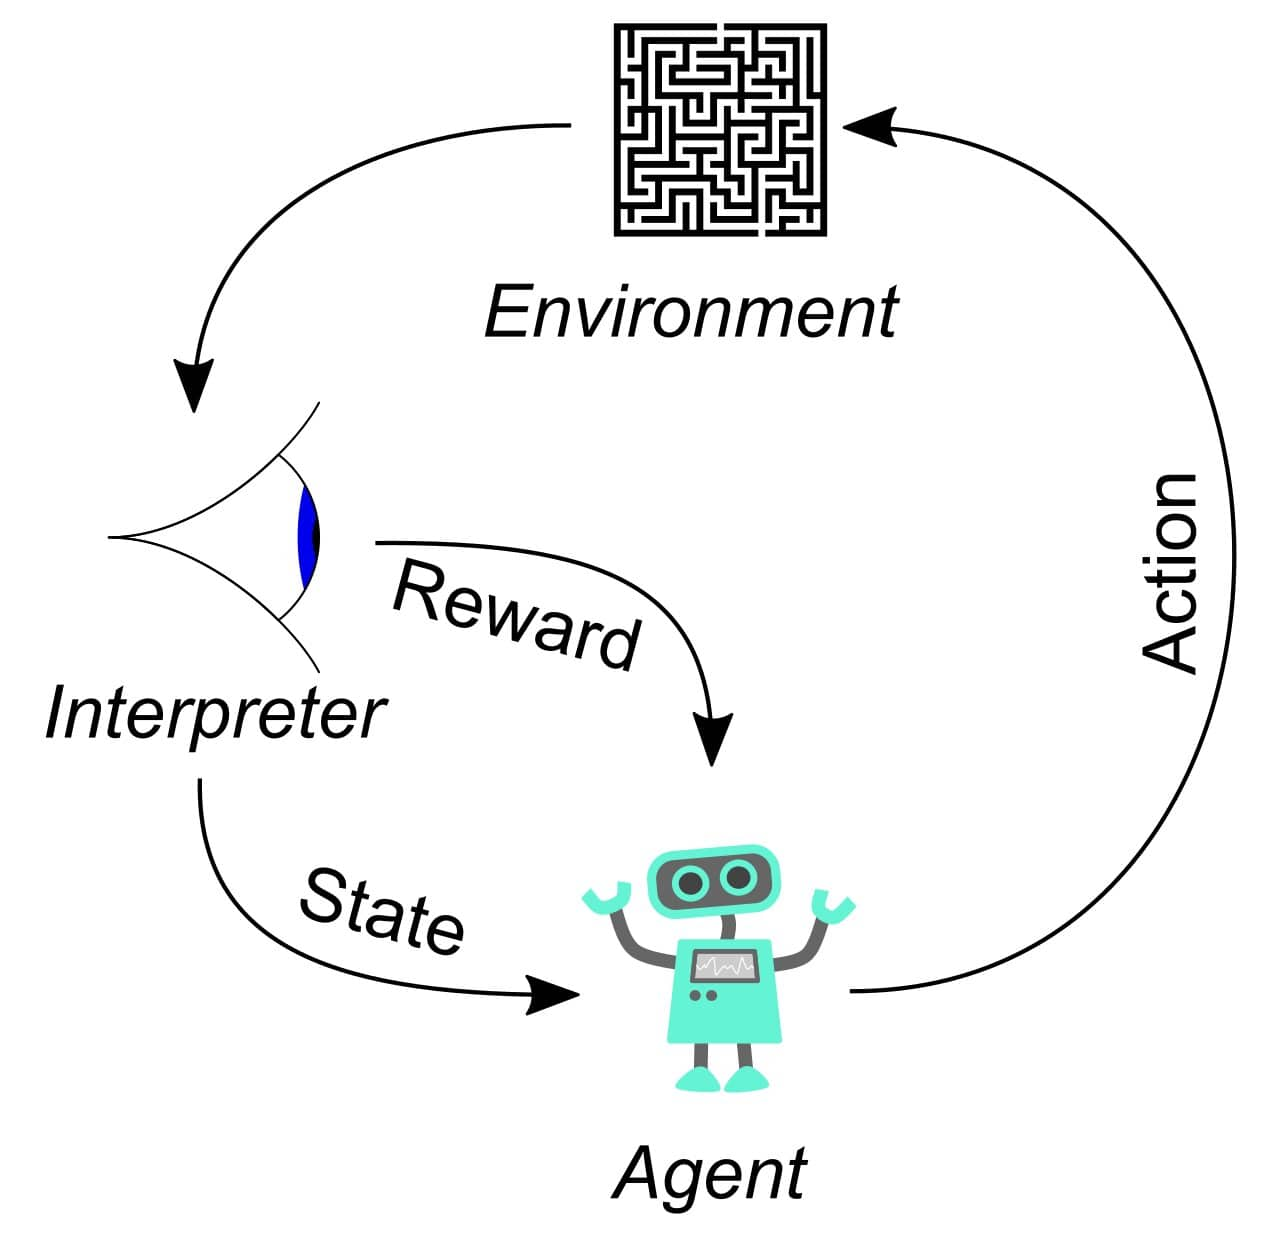
\includegraphics[width=0.35\textwidth]{chapters/chapter3/images/rl.jpg}
	\caption{Diagram of reinforcement learning
		\label{fig:rl-diagram}
	}
\end{figure}


\subsection{Exploration vs Exploitation}
\label{dsgn:sec:rl:expt-v-explor}
A key idea in RL is the problem of exploration vs exploration. This means that if we have an ennvironment, and a policy that dictates how we should navigate the environment, should always follow the policy, or should we deviate and try to find a better path resulting in a higher reward.

In this project we follow a method called $\epsilon$-greedy in which we explore forever, but with a linearly decreasing probability of random moves. We select random moves with a probability $\epsilon$ that is linearly decreasing over a set number of timesteps; below is the method for choosing the moves.

\begin{center}
	\begin{itemize}
		\item Choose random action with probability $\epsilon$
		\item With probability $1 - \epsilon$ select \vspace*{-9.25mm} action = $$\argmax_{a \in \mathcal{A}}~\hat{Q}(a)$$
	\end{itemize}
\end{center}

\section{Q-Learning}
\label{dsgn:sec:qlearning}

\section{Q-Learning improvements}
\label{dsgn:sec:qlearning:qextra}

\subsection{Double Q-Learning}
\label{dsgn:sec:qlearning:doubledqn}

\subsection{Duelling Q-Learning}
\label{dsgn:sec:qlearning:dueldqn}
